


\documentclass[conference]{IEEEtran}







\usepackage{acronym}


\usepackage{array}
\usepackage{multirow}
\usepackage{epsfig}
\usepackage{xspace}
\usepackage{url}
%\usepackage[dvips]{color}
\usepackage{subfigure}
\usepackage{pgf}
\usepackage{pgfplots,pgfplotstable} %for plotting results
\usepgfplotslibrary{units}
\usepackage{amsmath}
\usepackage{amsfonts,amssymb}
\usepackage{mathrsfs}
\usepackage{filecontents}
\usepackage{tikz} % for drawing
\usetikzlibrary{arrows,shapes,fit,automata,positioning,decorations,calc} % for drawing
\usetikzlibrary{spy,backgrounds}
\usepackage{algorithmic, algorithm}
\newcounter{lemmas}
\newtheorem{lemma}{Lemma}
%\newcounter{proofs}
%\newtheorem{proof}{Proof}
\newcounter{theorems}
\newtheorem{theorem}{Theorem}


%\newtheorem*{proof*}{Theorem}
%\newtheorem*{proof}{Proof}



\newcounter{definitions}
\newtheorem{definition}{Definition}

\input{./content/00_macros.tex}  %Macros/#defs for the paper
\begin{document}
\acrodef{CPS}{Cyber-Physical Systems}
\acrodef{DSP}{Digital Signal Processor}
\acrodef{DTTS}{Discrete Time Transition System}
\acrodef{DHA}{Deterministic Hybrid Automata}
\acrodef{EA}{Evolutionary Algorithm}
\acrodef{HA}{Hybrid Automata}
\acrodef{ILP}{Integer Linear Programming}
\acrodef{MCU}{Microcontroller Unit}
\acrodef{ODE}{Ordinary Differential Equation}
\acrodef{PoC}{Plant-on-a-Chip}
\acrodef{SHA}{Synchronous Hybrid Automata}
\acrodef{SWA}{Synchronous Witness Automata}
\acrodef{WHA}{Well-formed Hybrid Automata}
\acrodef{WCET}{Worst-Case Execution Time}
\acrodef{FSM}{Finite State Machine}

\acrodef{UP}{Upstroke}
\acrodef{ERP}{Effective Refractory Period}
\acrodef{RRP}{Relative Refractory Period}
\acrodef{RP}{Resting Period}
\acrodef{AP}{Action Potential}

\acrodef{SA}{Sinoatrial}
\acrodef{AV}{Atrioventicular}
\acrodef{RVA}{Right Ventricular Apex}


\acrodef{NHC}{Network of Heart Cells}
\acrodef{WH}{Water Heating System}
\acrodef{MTG}{Multiple Train Gate control}
\acrodef{TSN}{Thermostat Network}
\acrodef{NP}{Nuclear Plant control}
 		%acronyms
	
\title{Modular Code Generation from Hybrid Automata for Plant Emulation }

\author{
	%blind review
	%\IEEEauthorblockN{Nathan Allen, Sidharta Andalam, Partha Roop and Avinash Malik}
	%\IEEEauthorblockA{Department of Electrical and Computer Engineering \\
	%	University of Auckland, New Zealand\\
	%	Email: \{nall426, sand080, p.roop, avinash.malik\}@aucklanduni.ac.nz
	%}
}





\maketitle


\begin{abstract}
Real-time emulation of a plant is often desirable to facilitate the testing of controllers under realistic conditions.
Plants which exhibit continuous dynamics can be well modelled through the use of \acf{HA}, and so code generation from \ac{HA} that is suitable for real-time emulation is desirable.
In the case of plants which are modelled by a network of \acp{HA}, such code generation must be able to emulate the entire overall system through parallel composition.

In this paper, we propose a new tool (named \ourTool) for the modular code generation from \ac{HA} that is amenable to use in both the real-time emulation or simulation of plants.
We illustrate the suitability of this approach through the running example of a human heart, where real-time emulation is desired for the verification of cardiac pacemakers.
We compare the proposed approach to \simulink, a tool commonly used in the modelling of plants, to show that we are able to generate code that is on average 54\% smaller while executing 9.8 times faster.
We finish by showing the scalability of our approach in order to illustrate its potential in allowing real-time emulation of complex \ac{HA} networks.
\end{abstract}



\section{Introduction}

Pacemakers are safety-critical \acp{CPS} 
that control the pacing of a heart for providing therapy for bradycardia.
Such devices must operate in a fail-safe manner all the time.
However, between 1990-2000, close to 200,000 pacemakers have been recalled
due to software related failures~\cite{alemzadeh13}. Considering this,
 there is a need for the development of better processes for validation and 
certification of such devices. We propose the well known, and widely 
used, engineering technique of \emph{emulation}~\cite{patel2015survey}
 to tackle this problem. Emulation, also known as  hardware-in-the-loop simulation,
 is used to validate controllers (such as motor controllers) by running them in closed-loop
with the actual plant (the synchronous motor, for example). 
However, for emulation of pacemakers, the use of the actual plant (i.e. animal / human organs) is limiting.
Hence, there is a need for the development of high-fidelity heart models that 
 can provide the required real-time response to facilitate emulation. Bioengineering heart models~\cite{Trayanova2014}
 provide excellent model fidelity at the expense of computation time as the simulation of a single heart beat may take 
several hours. Hence, such models are not suitable for emulation.

Recently, timed automata~\cite{zhihao12} based heart models have been 
 developed primarily for model checking. These models 
abstract the continuous dynamics and hence unsuitable for emulation. 
In contrast to this, \acf{HA}~\cite{alur2015principles, raskin05} is used for modelling the forward conduction system
of the heart using 33 nodes in~\cite{chen14}. This work is the  starting point 
for real-time emulation by demonstrating that \simulink can be used for 
 closed-loop verification of pacemakers. However, this work has limited model 
fidelity and the limitations of the tool \simulink are inherited by the developed approach.
\simulink has semantic limitations, as the semantics of composition is unclear.
Moreover, there is no direct correspondence between the \simulink model and 
the \ac{HA}  models. Finally, \simulink generated code has scalability issues, due to which 
the researchers modelled a 33-node conduction system.

We develop an approach by combining node models (which are
extensions to the models developed by~\cite{chen14}) with 
 \emph{path models} (in timed automata) to accurately 
model the conduction delay between nodes. We are, thus, able to 
model the re-entrant behaviour of the heart. 

For modular code generation, we have developed an approach 
 based on the well known synchronous languages~\cite{benveniste03}.
 We formalise a deterministic subset of \ac{HA} called \ac{SHA}.
 Using the concept of delayed synchronous composition~\cite{boussinot96}, we are then able to
  produce modular code for each node separately. Such code has both code size and execution time
benefits for emulation. In addition, such code is based on semantic-preserving 
code generation, similar in spirit to Ptolemy~\cite{ptolemaeus2014system} and Z\'{e}lus~\cite{bourke13zelus}.
However, unlike our approach, these rely on dynamic numerical solvers, which is not ideal for emulation of the heart.
 
 \ignore{One reason that these malfunctions
arise is due to the lack of proper validation.
Unlike the ideas of hardware-in-the-loop testing,
also known as \emph {emulation}~\cite{patel2015survey},
it is not possible to test on an actual heart.
Further, unlike the hardware which is almost identical 
during mass production, each individual heart is different.
Thus there is a need to develop a virtual heart that is tailored
to an individual person and achieve
personalised healthcare~\cite{Trayanova2014}. 
This idea can be extended 
to a network of human organs, resulting in a virtual human.

Typically these biological  models are  developed by biomedical engineers.
They mimic the heart's working at the
molecular level~\cite{Trayanova2014}. 
To simulate one heart beat takes several hours, if not days.
These models are very computationally intensive and 
are not suitable for real-time emulation,
which is required for closed-loop testing of time-critical 
controllers such as cardiac pacemakers.
Further, the models are 
 very complex and hence 
 are not amenable for  formal verification. 
Thus, there is a need to develop abstract models 
by computer systems engineers that  
(1)  \emph{capture the behaviour} of the heart (plant) 
from a pacemaker's (controller's) point of view,
(2) \emph{allows for real-time emulation} of the heart 
such that it is possible for closed-loop simulation and
(3) \emph{are amenable for formal verification} of 
functional and timing properties.


The continuous dynamics of a plant (e.g. heart) and
 the discrete behaviour of a controller (e.g. pacemaker) 
 result in so called hybrid systems. 
 These are often formally described using \acf{HA}~\cite{alur2015principles,raskin05,chen201487}.
 However, these are non-deterministic and are problematic
 for generating constructive models.
 A more abstract deterministic model will enable us to
 develop constructive/synthesizable models~\cite{Lee2014}. Also, 
 it is easier to draw trusted conclusions from simulations
 of deterministic models. Based on the
 well-known synchronous approach~\cite{benveniste03}, 
 we present a deterministic semantics for \ac{HA} and show
 constructive models in this paper.


Traditional \ac{CPS} design uses commercial tools such as \simulink for plant simulation and emulation.
However, such designs do not preserve formal semantics of the models and are more verbose to describe.
Academic tools for code generation from \ac{HA} models such as Ptolemy~\cite{ptolemaeus2014system} and Z\'{e}lus~\cite{bourke13zelus}.
While these tools preserve the formal semantics, their reliance on dynamic numerical solvers makes them unsuitable for real-time emulation of plants.
Such tools are capable of expressing the full non-deterministic nature of \acp{HA} rather than the deterministic subset described here.}

   
 An overview of the proposed approach is presented
 in Figure~\ref{fig:overview}. Given a network
 of \acp{HA} for the nodes and paths of the conduction systems, the \ac{SHA} corresponding to these are generated. \ac{SHA} is an abstraction using the
synchronous approach to facilitate the generation of executable code (captured using \acp{FSM} for each node).
 
 \begin{figure}[bthp]
 	\centering
 	\scalebox{0.7}{
	 % Define block styles
\tikzstyle{decision} = [diamond, draw, fill=white!30, 
text width=5em, text badly centered, node distance=3.2cm, inner sep=0pt]
\tikzstyle{file} = [rectangle, draw, fill=gray!20, 
text width=5em, text centered, minimum height=4em]
\tikzstyle{process} = [rectangle, draw, fill=blue!15, 
text width=5em, text centered, rounded corners, minimum height=4em]
\tikzstyle{line} = [draw, -latex', ultra thick]
\tikzstyle{state} = [draw, ellipse,fill=red!30, 
node distance=3.5cm, text width=5em, 
text badly centered,
minimum height=2em]


\begin{tikzpicture}[node distance = 1cm, auto]
% Place nodes
\node [file] (HA) {{HA}};

\node [decision, right of = HA] (D) {Is a WHA~? (step 1,a
	Sec~\ref{sec:static-analysis-ha})};

\node [state, right of = D] (E) {Invalid input};

\node [file, right of = E, node distance=3cm] (FSM) {FSM/ C-code};


\node [process, below of = D, node distance =3cm] (GSHA) {Generate
	\ac{SHA} (step 2, Sec~\ref{sec:generation-sha})};

\node [file, below of = E, node distance =3cm] 
(SHA) {\ac{SHA}};

\node [process, below of = FSM, node distance =3cm] (GFSM)
{Generate backend code (step 3,
	Sec~\ref{sec:back-code-gener})};



%edges
\path [line] (HA) -- (D);
\path [line] (D)-- node[near start]{no}(E);
\path [line] (D)-- node[near start]{yes}(GSHA);

\path [line] (GSHA) -- (SHA);
\path [line] (SHA) -- (GFSM);
\path [line] (GFSM) -- (FSM);
\end{tikzpicture}    
	}
	 \caption{Overview of the proposed modular 
	 	code generation approach \label{fig:overview}}
\end{figure}
      
\textbf{Contributions} of this paper are 
(1) We propose a \emph{deterministic semantics} for \acf{HA}, see Section~\ref{sec:HA}.
We develop the electrical conduction system of the heart as a re-entrant circuit,
 using the proposed approach, as a case study.
(2) A \emph{scalable modular code generation} approach is developed, for the first time for \ac{HA} models, (Section~\ref{sec:codeGen}).
(3) We \emph{quantitatively evaluate} the efficacy of the 
proposed approach relative \simulink (Section~\ref{sec:benchmarking}).
 

\section{Background on Heart }
\begin{figure*}[htbp]
	\centering
	{
	\centering
	\subfigure[The four stages of an \acf{AP}]{
		\framebox[0.31\textwidth]{
			\begin{tikzpicture}[transform shape, xscale=0.6, yscale=0.6]
\begin{axis}
[ xlabel={Time (ms)},
ylabel={Potential ({mV})},
axis y line = left,
axis x line = bottom,
xmin=0,   xmax=300,
ymin=0,   ymax=150,
extra tick style={grid=major}
]
\addplot[color=blue!90,
mark=.,
mark size=2,
smooth,
const plot
]
table [x=t, y=v, col sep=comma] {./figures/actionPotentialData.csv};
\end{axis}

\tikzstyle{every state}=[rectangle, text centered, draw=none,text=black, draw,line width=0.3mm]

\node[state, shift={(0.55, -1.5)}, fill=green!20, minimum width=1.1cm] {RP};
\node[state, shift={(1.35, -1.5)}, fill=blue!20, minimum width=0.5cm] {UP};
\node[state, shift={(3.00, -1.5)}, fill=red!20, minimum width=2.8cm] {ERP};
\node[state, shift={(5.15, -1.5)}, fill=yellow!20, minimum width=1.5cm] {RRP};
\node[state, shift={(6.40, -1.5)}, fill=green!20, minimum width=1cm] {RP};

\end{tikzpicture}
			\label{fig:actionPotential}
		}
	} % HA
	\subfigure[\label{fig:heart} Diagram of the heart. The \acf{SA} node is the natural pacemaker of a heart]{
          \framebox[0.31\textwidth]{
				\includegraphics[width=0.30\linewidth]{figures/heart}
		} %framebox
	}% SHA
	\subfigure[An abstracted model of the conduction system as a network of $33$~nodes and conduction pathways in the Atria (Green) and Ventricles (Blue)]{ 
          \framebox[0.31\textwidth]{
          	\input{./figures/heartNetwork.tex}
          	\label{fig:heartNetwork} 
	  } %framebox
	}% code gen

}
	\caption{Electrical conduction systems of a heart}
	\label{fig:heartOverview}
\end{figure*}

In this section, using Figure~\ref{fig:heartOverview} we 
describe the electrical conduction system of the heart.

\noindent \textbf{Heart.}
The human heart (see Figure~\ref{fig:heart})
 is an organ that pumps blood throughout the body.
It achieves this by regularly contracting an relaxing the muscles
which are orchestrated by a flow of electrical signals through the heart.
The signal is primarily generated automatically by the \ac{SA} node.
First, the signal travels through left and right atrium, contracting 
the muscles and pushing the blood into ventricles.
 
Second, to ensure the both ventricles are filled, 
the \ac{AV} node introduces critical delay 
in the conduction system.   
Finally, the electrical signal propagates through 
both ventricles. This contracts the muscles and pumps the blood out.


	
\noindent \textbf{\acf{AP}.} 
The propagation of electrical signal at cellular level 
is described as a change in  voltage 
across cell membrane due to ionic flow over a period of time, 
know as \acf{AP} shown in Figure~\ref{fig:actionPotential}. 
The voltage behaviour can be described in four stages.
\begin{enumerate}
	\item \acf{RP}: This is the steady state of the cell and awaits for 
					external stimulus current to activate it.
	\item \acf{UP}: When activated by stimulus current, 
					the cell depolarises (inward flow of positive ions) and 
					contracts the muscles. This depolarisation yields 
					stimulus current that activates neighbouring cells.
	\item \acf{ERP}: Once activated, the cell cannot be activated again 
					 due to recovery process of the ionic channels. 
					 Any new stimulus will be blocked. 
	\item \acf{RRP}: During this period, the ionic channels are partially recovered
					 and the cell can be activated. However, the morphology
					 of the action potential curve will be shorter.
	
\end{enumerate} 
 For more details on understanding \acp{AP} please refer to~\cite{chen14}.\\

\noindent \textbf{Abstract model.}
The human heart has over two trillion cells. For analytical purposes, a
model consisting a network of $32$ nodes is presented in literature
and is used for testing off-the-shelf pacemakers~\cite{chen14,zhihao12}.
The abstracted electrical conduction system consisting  of 
nodes and paths is presented in Figure~\ref{fig:heartNetwork}.
The functionality of each node is described using \acf{HA} in Section~\ref{sec:HA}. The path model describes the 
conduction delay of the electrical signal.
Later in Section~\ref{sec:codeGen}, we use the abstract network model 
to illustrate our modular code generation.

 

\section{Hybrid Automata}
\label{sec:HA}



\acf{HA} is ideal for describing 
Cyber-physical systems. As explained in the Introduction,
non-deterministic of \ac{HA} are not suitable for modelling and
emulation of a plant. To address this problem, based on the
synchronous approach~[], we propose a deterministic semantics for \ac{HA}.
In this section, we (1) present an example \ac{HA} 
followed by a formal definition.
Then, we present deterministic semantics for \ac{HA} 
along with a proof for determinism.



\subsection{Example of \ac{HA} (TEXT NEEDS TO BE UPDATED)}

\begin{figure}
\centering
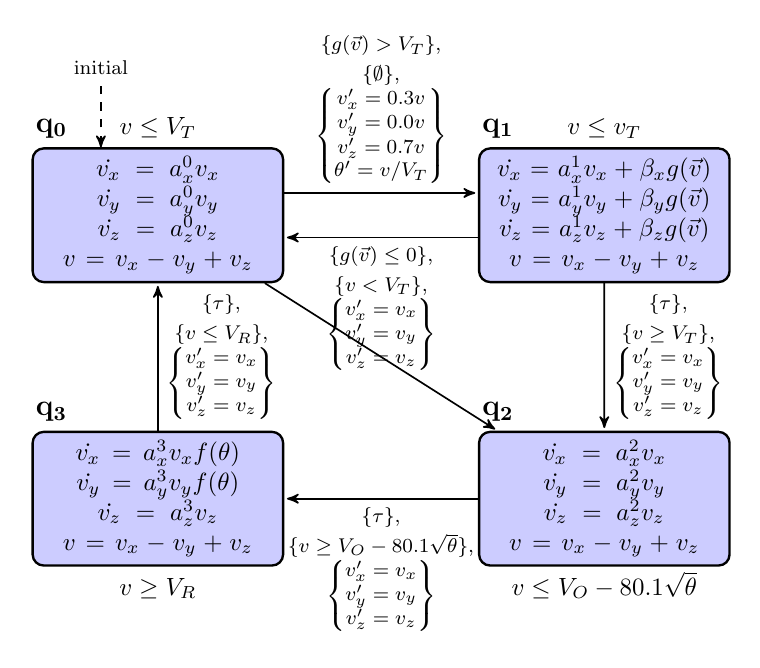
\begin{tikzpicture}[->,>=stealth',shorten >=1pt,auto,
node distance=4cm,
semithick,scale=0.9, transform shape]
\tikzstyle{every state}=[rectangle,rounded corners,
 minimum height = 1.2cm, text width=3.3cm, text centered, fill=blue!20,draw=none,text=black, draw,line width=0.3mm]

\node[state, 
label={[shift={(0,0)}]$v \leq V_T$}, 
label={[shift={(-1.5,0)}]\large $ \mathbf{q_0}$ }]
(Q0)  {$\dot{v_x}=a^0_x v_x$ \\ $\dot{v_y}=a^0_y v_y$ \\ $\dot{v_z}=a^0_z v_z$ \\ $v=v_x - v_y + v_z$};

%entry
\draw[<-, dashed](Q0.130) -- node[above, shift={(0,0.4)}] {\footnotesize initial} ++(0cm,1cm);




\node[state, 
label={[shift={(0,0)}]$v \leq v_T$}, 
label={[shift={(-1.5,0)}]\large $\mathbf{q_1}$   }]
(Q1) [node distance=6.3cm, right of=Q0] {$\dot{v_x}=a^1_x v_x + \beta_x g(\vec{v})$ \\ $\dot{v_y}=a^1_y v_y + \beta_y g(\vec{v})$ \\ $\dot{v_z}=a^1_z v_z + \beta_z g(\vec{v})$ \\ $v=v_x - v_y + v_z$};

\node[state, 
label={[shift={(0,-2.5)}]$v \leq V_O - 80.1 \sqrt{\theta}$}, 
label={[shift={(-1.5,0)}]\large $\mathbf{q_2}$  }] 
(Q2) [below of=Q1] {$\dot{v_x}=a^2_x v_x$ \\ $\dot{v_y}=a^2_y v_y$ \\ $\dot{v_z}=a^2_z v_z$ \\ $v=v_x - v_y + v_z$};

\node[state, 
label={[shift={(0,-2.5)}]$v \geq V_R$}, 
label={[shift={(-1.5,0)}]\large $\mathbf{q_3}$  }]
(Q3) [below of=Q0] {$\dot{v_x}=a^3_x v_x f(\theta)$ \\ $\dot{v_y}=a^3_y v_y f(\theta)$ \\ $\dot{v_z}=a^3_z v_z$ \\ $v=v_x - v_y + v_z$};

\path[->] (Q0.10) edge node[align=center] {
	\footnotesize $\{g(\vec{v}) > V_T\}$, \\
	\footnotesize $\{\emptyset\}$, \\
	\footnotesize $\left\{\begin{matrix} v^\prime_x = 0.3v \\ v^\prime_y = 0.0v \\ v^\prime_z = 0.7v \\ \theta^\prime = v / V_T \end{matrix}\right\}$
} (Q1.170);

\path[->] (Q1.190) edge node[align=center] {
	\footnotesize $\{g(\vec{v}) \leq 0\}$, \\
	\footnotesize $\{v < V_T\}$, \\
	\footnotesize $\left\{\begin{matrix} v^\prime_x = v_x \\ v^\prime_y = v_y \\ v^\prime_z = v_z \end{matrix}\right\}$
} (Q0.350);

\path[->] (Q1) edge node[align=center] {
	\footnotesize $\{\tau\}$, \\
	\footnotesize $\{v \geq V_T\}$, \\
	\footnotesize $\left\{\begin{matrix} v^\prime_x = v_x \\ v^\prime_y = v_y \\ v^\prime_z = v_z \end{matrix}\right\}$
} (Q2);

\path[->] (Q2) edge node[align=center] {
	\footnotesize $\{\tau\}$, \\
	\footnotesize $\{v \geq V_O - 80.1\sqrt{\theta}\}$, \\
	\footnotesize $\left\{\begin{matrix} v^\prime_x = v_x \\ v^\prime_y = v_y \\ v^\prime_z = v_z \end{matrix}\right\}$
} (Q3);

\path[->] (Q3) edge node[align=center, shift={(1.8,0)}] {
	\footnotesize $\{\tau\}$, \\
	\footnotesize $\{v \leq V_R\}$, \\
	\footnotesize $\left\{\begin{matrix} v^\prime_x = v_x \\ v^\prime_y = v_y \\ v^\prime_z = v_z \end{matrix}\right\}$
} (Q0);

\draw[->](Q0)--(Q2);

\end{tikzpicture}
\caption{\acf{HA} of a heart cell}
\end{figure}

An HA~\cite{lynch03} is defined using Definition~\ref{def:ha}. For the
water tank example shown in Figure~\ref{fig:waterTankHAtank},
$Loc=\{t_1, t_2, t_3, t_4\}$, $\Sigma=\{ON, OFF, \tau\}$, and an example
edge in $Edge$ is $(t_1, ON, t_2)$. There is a single continuous
variable $x$ representing the temperature of the water in the
tank. Hence, $X=\{x\}$, $\dot{X}=\{\dot{x}\}$, and $X'=\{x'\}$. The only
location that is marked initial is $t_1$ and $Init(t_1): x=20$. An
example flow predicate is $Flow(t_1): \dot{x}=0$, which specifies that
the temperature of the water inside the tank does not change.  A jump
predicate assigned to an edge specifies the condition needed to take a
transition and the updating of values of some continuous variables when
the transition is taken.  For example,
$Jump(t_4, \tau, t_1): x=20 \wedge x'=x$ specifies that the transition
is taken when the value of the temperature is $20^\circ$C and the
updated value of the temperature is also $20^\circ$C. We now formalise
the HA using Definition~\ref{def:ha}.

\subsection{Definition of \ac{HA}}

\begin{definition}
	A hybrid automata is \newline 
	$H = \langle Loc, Edge, \Sigma, Inv, Flow, Jump \rangle$ where
	\begin{itemize}
		\item $Loc=\{l_1,..,l_n\}$ representing $n$ control modes or
		locations.
		\item $Edge \subseteq Loc \times \Sigma \times Loc$ are the set of
		edges between locations.
		\item $\Sigma=\Sigma_I \cup \Sigma_O \cup \{\iSignal\}$ is set of
		event names comprising of input, output, and internal events.
		\item Three sets for the set of continuous variables, their rate of
		change and their updated values represented as follows: \newline
		$X=\{x_1,.., x_m\}$, $\dot{X}=\{\dot{x_1},.., \dot{x_m}\}$, and \newline
		$X'=\{x_{1}',.., x_{m}'\}$.
		\item $Init(l)$: Is a predicate whose free variables are from $X$. It
		specifies the possible valuations of these when the HA starts in
		$l$.
		\item $Inv(l)$: Is a predicate whose free variables are from $X$ and
		it constrains these when the HA resides in $l$.
		\item $Flow(l)$: Is a predicate whose free variables are from
		$X \cup \dot{X}$ and it specifies the rate of change of these
		variables when the HA resides in $l$.
		\item $Jump(e)$: Is a function that assigns to the edge `$e$' a
		predicate whose free variables are from $X \cup X'$. This predicate
		specifies when the mode switch using `$e$' is possible. It also
		specifies the updated values of the variables when this mode switch
		happens.
	\end{itemize}
	\label{def:ha}
\end{definition}


\subsection{Deterministic semantics of \ac{HA}}

\subsection{Proof for determinism}
\section{Modular code generation}
\label{sec:codeGen}

In this section we present our approach for modular code generation from a network of \acp{HA}. 
An overview of the solution is presented in Figure~\ref{fig:overview}, with the first of the two steps being outlined in Section~\ref{sec:shaGeneration}, and the second step in Section~\ref{sec:backendCodeGeneration} below.



\subsection{Backend code generation}
\label{sec:backendCodeGeneration}

Secondly, we describe step $2$ of the compilation process from Figure~\ref{fig:compilingHA}. Once a network of \acp{SHA} has been created,...

\begin{itemize}
	\item code generation
	\item composition
	\item Proof for Determinism (still holds ?)
\end{itemize}

\begin{figure}
	\centering
	\input{figures/cellFSM}
	\caption{\acf{FSM} of a heart cell \label{fig:heartCellFSM}}
\end{figure}


\begin{figure}
	\centering
	\input{figures/cellComposition}
	\caption{Synchronous composition of multiple heart cells \label{fig:heartCellComposition}}
\end{figure}
\section{Benchmarking}
\label{sec:benchmarking}


We present a set of experiments to evaluate the efficacy of the proposed modular code generation tool (\ourTool) with \simulink. 
In the first experiment, we select benchmarks that span across different application domains such as medical, physics, and industrial automation, to illustrate the \emph{diversity} of the proposed approach.
We then compare each of these benchmarks against \simulink in terms of execution time and maximum memory usage.
In the second experiment, we evaluate the \emph{scalability} of \ourTool and \simulink as the number of cells in the \ac{NHC} model increases. 


\subsection{Experimental set-up}
\label{sec:experimentalSetUp}
The following steps were considered in order to achieve a fair comparison between \ourTool and \simulink:

\begin{description}[\IEEEsetlabelwidth{Step Size}\IEEEusemathlabelsep]
	\item[\textbf{Solver}] To reflect the synchronous execution model, we used a discrete solver with a fixed step in \simulink, namely \texttt{ode1} (Forward Euler).
	
	\item[\textbf{Step Size}] For all benchmarks the step size in \simulink is fixed to $0.01$ milliseconds.
	The same step size is also used in \ourTool, $\delta = 0.01$ milliseconds.
	
	\item[\textbf{Time}] All benchmarks were simulated for $10$ seconds of simulation time.
	Based on a step size of $0.01$ milliseconds this translates to $1$ million ticks in \ourTool.
\end{description}

The experiments were evaluated using an Intel~i7-4790 processor with 8~GB RAM on Windows~7. 


\subsection{Diversity}

\begin{figure}[htbp]
	\centering
	\subfigure[Execution time (ms) \label{fig:executionTime}]{
		\begin{tikzpicture}
\begin{axis}[
	ybar,
	enlargelimits=0.15,
	legend style={
		at={(0.5,-0.15)},
		anchor=north,
		legend columns=-1
	},
	ylabel={Execution time (ms)},
	symbolic x coords={TSN, NHC, WH, MTG, NP},
	xtick=data,
	nodes near coords,
	nodes near coords align={vertical},
]

%Simulink
\addplot coordinates {
	(TSN,0)
	(NHC,14254)
	(WH,0)
	(MTG,0)
	(NP,0)
};

%Piha (O0)
\addplot coordinates {
	(TSN,316)
	(NHC,1997)
	(WH,0)
	(MTG,249)
	(NP,504)
};

%Piha (O2)
\addplot coordinates {
	(TSN,119)
	(NHC,713)
	(WH,0)
	(MTG,113)
	(NP,207)
};

\legend{\simulink, \ourTool (O0), \ourTool (O2)}

\end{axis}
\end{tikzpicture}

	}
	\subfigure[Memory requirement (MB) \label{fig:memoryRequirement}]{
		\input{./figures/memoryRequirementGraph}
	}
	\caption{Comparison of the execution time (in ms) and memory requirement (in MB) between \simulink and \ourTool for the benchmarks in Table~\ref{tab:benchmarks}.}
	\label{fig:results}
\end{figure}

For the purposes of this experiment, we use the five benchmarks presented in Table~\ref{tab:benchmarks}.
The table also presents the number of locations (\#L) in each hybrid automata.
For example, $(2, 2, 2)$ denotes that the \acf{TTS} benchmark is described using three \acp{HA} each with two locations.
More details about the benchmarks and their implementation in \ourTool and \simulink are available online~\cite{githubBenchmarks}.

For all the benchmarks, the executable for the \simulink models are generated using the in-built Real-time Workshop\textsuperscript{\textregistered} C code generator.
Similarly, for \ourTool, we generate equivalent C code and compile to an executable using GCC.
The execution times and memory requirements of the generated executables are reported below and illustrated in Figure~\ref{fig:results}.

\textbf{Execution time:} 
Figure~\ref{fig:executionTime} shows that...

\textbf{Code size:}
Figure~\ref{fig:memoryRequirement} shows that...

On average, the code generated by \ourTool executes ?? times faster, while requiring ?? times less memory when compared to \simulink.

\begin{table*}
	\centering
	\caption{Benchmark descriptions
	\label{tab:benchmarks}}
\begin{tabular}{ | c | c | c | l | } \hline
\textbf{Benchmarks}
	& \textbf{Domain} 
	& \textbf{\#L } 
	& \textbf{Description} \\ \hline

	\acf{TTS}
		& Physics~\cite{Pedro2005}
		& $(2, 2, 2)$
		& Three thermostats heating a room to keep it warm\\ \hline
		
	\acf{NHC}
		& Biology~\cite{chen201487}
		& $(4, 4, ..., 4)$
		& Captures the electrical conduction system of a heart with $33$ nodes\\ \hline

	\acf{WH}
		& Physics~\cite{raskin05}
		& $(4, 4)$
		& Models the heating of water in a tank \\ \hline
		
	\acf{MTG}  
		& Industrial automation~\cite{Costello2013}
		& $(2, 3, ..., 3)$
		& Models the behaviour of a gate and $30$ trains at a rail road crossing\\ \hline
		
	\acf{NP}
		& Industrial automation~\cite{alur2015book}
		& $(3, 3)$
		& Switches between two fuel rods to avoid nuclear meltdown\\ \hline
	
	
 \end{tabular}
 \end{table*}


\subsection{Scalability}

\begin{figure}[htbp]
	\centering
	\begin{tikzpicture}
\begin{axis}
[ xlabel={Number of Heart Cells},
ylabel={Execution Time ({s})},
axis y line = left,
axis x line = bottom,
xmin=0000,   xmax=1000,
ymin=0,
extra tick style={grid=major}
]
\addplot[color=blue!90,
mark=.,
mark size=2,
smooth
]
table [x=n, y=t, col sep=comma] {./figures/scalabilityGraphData.csv};
\end{axis}
\end{tikzpicture}
	\caption{Scalability in  execution time of \simulink and \ourTool against number of cells}
	\label{fig:scalability}
\end{figure}

The purpose of the second experiment was to validate the scalability of \ourTool through the running example of the \ac{NHC} whilst comparing it to \simulink.
Code was generated for varying network sizes (33 cells, 66 cells, 99 cells, etc.) and the execution time recorded.
The experimental set-up was the same as described in Section~\ref{sec:experimentalSetUp}, ie. $1$ million ticks at a $0.01$ millisecond step size.

The most obvious feature of these results is that no data is recorded for \simulink for complexities greater than 297 cells. \simulink imposes an inbuilt requirement that the generated code use less than 2.1GB of memory and this discontinuity represents the point after which the memory requirement exceeds this limit\footnote{\simulink memory usage at 297 cells is 1.8GB}.

\begin{itemize}
	\item \ourTool has a smaller gradient
	\item \ourTool carries past this point that \simulink doesn't
	\item Point out the change in gradient around ~240 cells in \ourTool is due to cache size
	\item Mention the real time requirements for \ourTool vs \simulink
\end{itemize}
\section{Related work}
\label{sec:lit}
There are many solutions for code generation from \acf{HA}...
\begin{itemize}
	\item Upenn timed automata
	\item Simulink
	\item ....
\end{itemize}
\section{Conclusions}

While this paper focuses on the example of cardiac pacemakers.
The proposed code generation for emulation of plant is applicable 
beyond medical domain.
We show this during the experiments in Section~\ref{sec:benchmarking}.


For the hear model, while maintaining real-time response,
 we were able to emulate more than 200 nodes. In contrast,
 the Simulink tool was only capable of emulating 20 nodes. 
 This shows the proposed emulation approach is much superior than 
 the popular Simulink tool.


Talk about the limitation of our work



\bibliographystyle{ieeetr}
\bibliography{references} 

\end{document}


